\documentclass[10pt,twocolumn]{article}
\usepackage[margin=0.75in,columnsep=0.25in]{geometry}
\usepackage{booktabs}
\usepackage{graphicx}
\graphicspath{{../figures/}{figures/}}
\usepackage{amsmath, amssymb}
\usepackage{microtype}
\usepackage[font=small,labelfont=bf]{caption}
\usepackage[breaklinks=true,colorlinks=true,linkcolor=black,citecolor=black,urlcolor=blue]{hyperref}

\newcommand{\method}{IterAlign-LoRA}
\newcommand{\modelname}{SmolLM-135M}
\newcommand{\dataset}{DangerousQA}
\newcommand{\etal}{\textit{et al.}}

\title{\textbf{Parameter-Efficient Iterative Constitutional Alignment for Small Language Models}}
\author{Final Project Report -- Group ID 04, Project 5\\
Department of Artificial Intelligence and Data Science\\
School of Computing, FAST-NUCES}
\date{}

\begin{document}
\twocolumn[
\begin{@twocolumnfalse}
\maketitle
\begin{abstract}
Large language models can produce unsafe, dishonest, or policy-violating responses when prompted adversarially. Reinforcement learning from human feedback improves this behavior, but it requires preference labels, reward-model training, and substantial compute. Constitutional AI reduces part of the annotation cost by using model feedback under written rules, but the constitution still has to be supplied manually. IterAlign addresses this gap by inducing constitutions from a model's own failures: red-team prompts expose unsafe responses, a stronger oracle identifies harmful cases, the oracle induces rules from those failures, and the base model is fine-tuned on revised responses. This project studies IterAlign across three stages: paper understanding, reproduction, and extension. We reproduced a small-model IterAlign path using \texttt{HuggingFaceTB/SmolLM-135M}, Hugging Face Transformers, and Gemini 3.1 Flash Lite as oracle and judge. The reproduced full-fine-tuning baseline improved Gemini-judge score from 0.23 for the vanilla model to 0.42 on hh-rlhf, 0.45 on HarmfulQA, and 0.46 on \dataset. We then proposed \method, replacing full supervised fine-tuning with LoRA adapter training while preserving the red-team, oracle, constitution-induction, and revised-answer generation loop. \method{} reached 0.38, 0.41, and 0.42 on the same datasets after about four days, compared with roughly seven days for full fine-tuning. The extension sacrificed 0.04 judge-score points per dataset while reducing the training schedule by about 43\% and lowering estimated peak VRAM from about 2.5--3.5 GB to about 0.9--1.5 GB. Adapter tuning did not fully replace full fine-tuning, but it preserved most of the alignment gain in this course-scale reproduction.
\end{abstract}

\noindent\textbf{Keywords:} language model alignment, IterAlign, constitutional AI, LoRA, PEFT, red teaming, harmfulness evaluation, SmolLM.
\vspace{0.35in}
\end{@twocolumnfalse}
]

\section{Introduction}
\label{sec:introduction}

The safety behavior of a language model is not fixed by pretraining alone. A model trained only to predict the next token may produce harmful instructions, biased reasoning, dishonest statements, or evasive responses when prompted adversarially. Alignment methods try to shift this behavior toward helpfulness, harmlessness, honesty, and compliance with user intent. The standard route is reinforcement learning from human feedback (RLHF), where humans compare candidate outputs and a reward model learns the preference signal~\cite{ouyang2022instructgpt}. RLHF works well, but it is expensive to reproduce because it requires data collection, reward-model training, and reinforcement-learning optimization.

Constitutional AI (CAI) reduces part of that annotation burden by replacing many human preference labels with AI feedback under a written constitution~\cite{bai2022cai}. A model critiques and revises its own outputs according to a list of principles. This reduces labeling effort, but the constitution is still manually chosen. The resulting system depends on whether the written rules match the model's actual failure modes. A static constitution can miss errors that are specific to a model, prompt distribution, or deployment setting.

IterAlign proposes a data-driven alternative~\cite{chen2024iteralign}. Instead of starting with a fixed set of rules, the method first elicits failures through red-team prompts, asks a stronger oracle to identify negative responses, induces constitutions from those failures, and fine-tunes the model on safer revised responses. The constitution is derived from what the current model actually does wrong. IterAlign therefore combines red teaming, AI feedback, and supervised fine-tuning into one iterative loop.

Our final project examines IterAlign through the full assignment sequence. Assignment 1 focused on the original paper and its relationship to RLHF and CAI. Assignment 2 reproduced the method at a smaller scale using \modelname{} rather than the larger Llama-2 setup. Assignment 3 extended the reproduced pipeline with parameter-efficient fine-tuning. This final report combines those stages and reports both reproduced and additional experiments.

\textbf{Research gap.} IterAlign reduces the need for hand-written constitutions, but its iterative full fine-tuning loop remains expensive for small research environments. If every constitution-discovery round requires full-model updates, the method becomes harder to rerun across datasets, seeds, and low-resource hardware. The alignment loop is reproducible in principle, but the training update can still limit reproducibility in practice.

We address this gap by replacing the full fine-tuning step with Low-Rank Adaptation (LoRA)~\cite{hu2022lora} implemented through Hugging Face PEFT~\cite{peft2022}. The proposed method, \method, leaves the red-team prompts, oracle classifier, constitution-induction prompt, revised-answer generation, and Gemini-judge evaluation unchanged. It only changes the parameter update. The experiment asks whether adapter tuning preserves most of the safety improvement while reducing training cost.

The project contributes:
\begin{itemize}
  \item It summarizes IterAlign as a constitution-discovery pipeline and explains the difference between the paper-faithful implementation and the small-model reproduction path.
  \item It reports a reproduced \modelname{} baseline where full IterAlign fine-tuning improves Gemini-judge score from 0.23 to 0.42--0.46 across harmfulness datasets.
  \item It introduces a PEFT/LoRA extension that trains approximately 1.84M adapter parameters instead of updating the full base model.
  \item It compares full fine-tuning and LoRA across hh-rlhf, HarmfulQA, and the additional \dataset{} dataset, showing a consistent 0.04 score gap for about three fewer training days.
\end{itemize}

Section~\ref{sec:related} reviews related work. Section~\ref{sec:architecture} describes the proposed architecture. Section~\ref{sec:methodology} gives the methodology, equations, and algorithm. Section~\ref{sec:setup} describes the experimental setup. Section~\ref{sec:results} presents results and analysis. Section~\ref{sec:discussion} discusses limitations and implications, and Section~\ref{sec:conclusion} concludes.

\section{Background and Related Work}
\label{sec:related}

\subsection{Human-feedback alignment}
Ouyang \etal{} introduced InstructGPT, an RLHF pipeline for aligning language models to user intent~\cite{ouyang2022instructgpt}. The pipeline first trains a supervised model on demonstrations, then trains a reward model from human rankings, and finally optimizes the policy using reinforcement learning. For this project, the relevant result is that alignment data can matter more than scale alone. The limitation is cost: RLHF needs human preference labels and a reward-model training stage. For a course project, faithful RLHF reproduction is unrealistic.

Related instruction-following systems such as Llama 2 and Vicuna demonstrate that supervised and preference-based alignment can strongly shape assistant behavior~\cite{touvron2023llama2,vicunabench2023}. These systems are useful reference points because they show how much post-training affects chat behavior. They do not solve the narrower problem studied here: how to discover alignment rules from observed failures and then update a small model efficiently.

\subsection{Constitutional and AI-feedback alignment}
Bai \etal{} proposed Constitutional AI, where models critique and revise responses according to written principles and then use AI feedback for preference learning~\cite{bai2022cai}. CAI reduces the need for human labels, but it still assumes that a suitable constitution is available. IterAlign builds directly on this idea while changing the source of the constitution: rules are induced from harmful outputs rather than supplied in advance~\cite{chen2024iteralign}.

The distinction matters for reproducibility. A manually written constitution is easy to inspect, but it may not match a small model's actual errors. An induced constitution can adapt to the prompt distribution and model checkpoint. The cost is that a stronger oracle model remains necessary. In our reproduction, Gemini 3.1 Flash Lite acts as both oracle and judge. This substitution makes the run feasible, but it also means our absolute numbers are not directly comparable to the original paper's oracle setting.

\subsection{Red teaming and harmfulness benchmarks}
Red teaming deliberately searches for prompts that trigger unsafe or undesirable model behavior. Ganguli \etal{} released red-team attacks and documented how harmfulness behavior changes with model scale and alignment method~\cite{ganguli2022redteam}. Bhardwaj and Poria studied red-teaming large language models through chained utterances for safety alignment~\cite{bhardwaj2023redteaming}. These works treat red teaming mainly as a diagnostic and stress-testing tool. IterAlign uses it as a data source: failures are converted into constitutions and revised training targets.

This project uses three harmfulness-oriented prompt sources: an hh-rlhf red-team pool, HarmfulQA, and \dataset. \dataset{} is used as the additional experiment required for Assignment 3. The datasets are not treated as classification datasets with fixed labels. Instead, they provide prompts that drive model generation and oracle evaluation. This design matches the IterAlign loop, where the relevant unit is a prompt-response pair judged by an oracle.

\subsection{Parameter-efficient fine-tuning}
Full fine-tuning updates all model parameters and stores gradients and optimizer states for each trainable weight. LoRA reduces this cost by freezing pretrained weights and inserting trainable low-rank matrices into selected linear layers~\cite{hu2022lora}. QLoRA extends this efficiency direction by using quantized base weights and LoRA adapters~\cite{dettmers2023qlora}. PEFT libraries make these techniques easy to apply in Hugging Face training loops~\cite{peft2022}.

Parameter-efficient fine-tuning is particularly relevant to IterAlign because the method repeats training after constitution discovery. A one-time full fine-tune may be acceptable; repeated full fine-tuning across datasets or seeds becomes much more expensive. LoRA changes the cost profile by training only adapter parameters. The risk is reduced capacity. If safety improvements require broad movement in the base model's weights, adapters may not match full fine-tuning.

\subsection{Small language models and implementation tools}
The original IterAlign paper used larger language models and a heavier serving/training stack. Our reproduction uses \modelname{} from Hugging FaceTB~\cite{allal2024smollm}, Hugging Face Transformers~\cite{wolf2020transformers}, and PEFT~\cite{peft2022}. Smaller models make the project runnable in a course setting but change the interpretation of results. We compare full fine-tuning and LoRA under the same small-model setup rather than claiming direct equivalence with the original paper's large-model results.

Table~\ref{tab:related} summarizes the related approaches by method family. This organization matches the project contribution: the constitution-discovery loop is kept intact, while the fine-tuning mechanism changes.

\begin{table*}[t]
\centering
\caption{Related approaches and their relevance to this project.}
\label{tab:related}
\resizebox{\textwidth}{!}{%
\begin{tabular}{llll}
\toprule
Approach & Main idea & Limitation for this project & Relation to our work \\
\midrule
RLHF~\cite{ouyang2022instructgpt} & Human preference reward model & Requires preference data and RL & Motivates lower-cost alignment \\
Constitutional AI~\cite{bai2022cai} & AI feedback under written rules & Constitution must be predefined & Basis for rule-guided revision \\
Red teaming~\cite{ganguli2022redteam} & Probe models for harmful outputs & Primarily diagnostic by itself & Supplies failure cases for IterAlign \\
IterAlign~\cite{chen2024iteralign} & Induce constitutions from failures & Repeated full SFT is costly & Reproduced baseline and target method \\
LoRA~\cite{hu2022lora} & Low-rank trainable adapters & May underfit full-model changes & Proposed update mechanism \\
QLoRA~\cite{dettmers2023qlora} & Quantized LoRA fine-tuning & Adds quantization complexity & Future efficiency extension \\
\bottomrule
\end{tabular}%
}
\end{table*}

\section{Proposed Architecture}
\label{sec:architecture}

\subsection{System components}
The proposed system is not a new base transformer architecture. It is an alignment architecture built around five components: a base causal language model, a red-team prompt source, an oracle judge, a constitution-induction prompt, and a fine-tuning module. Figure~\ref{fig:pipeline} shows the architecture used across the project.

\begin{figure*}[t]
\centering
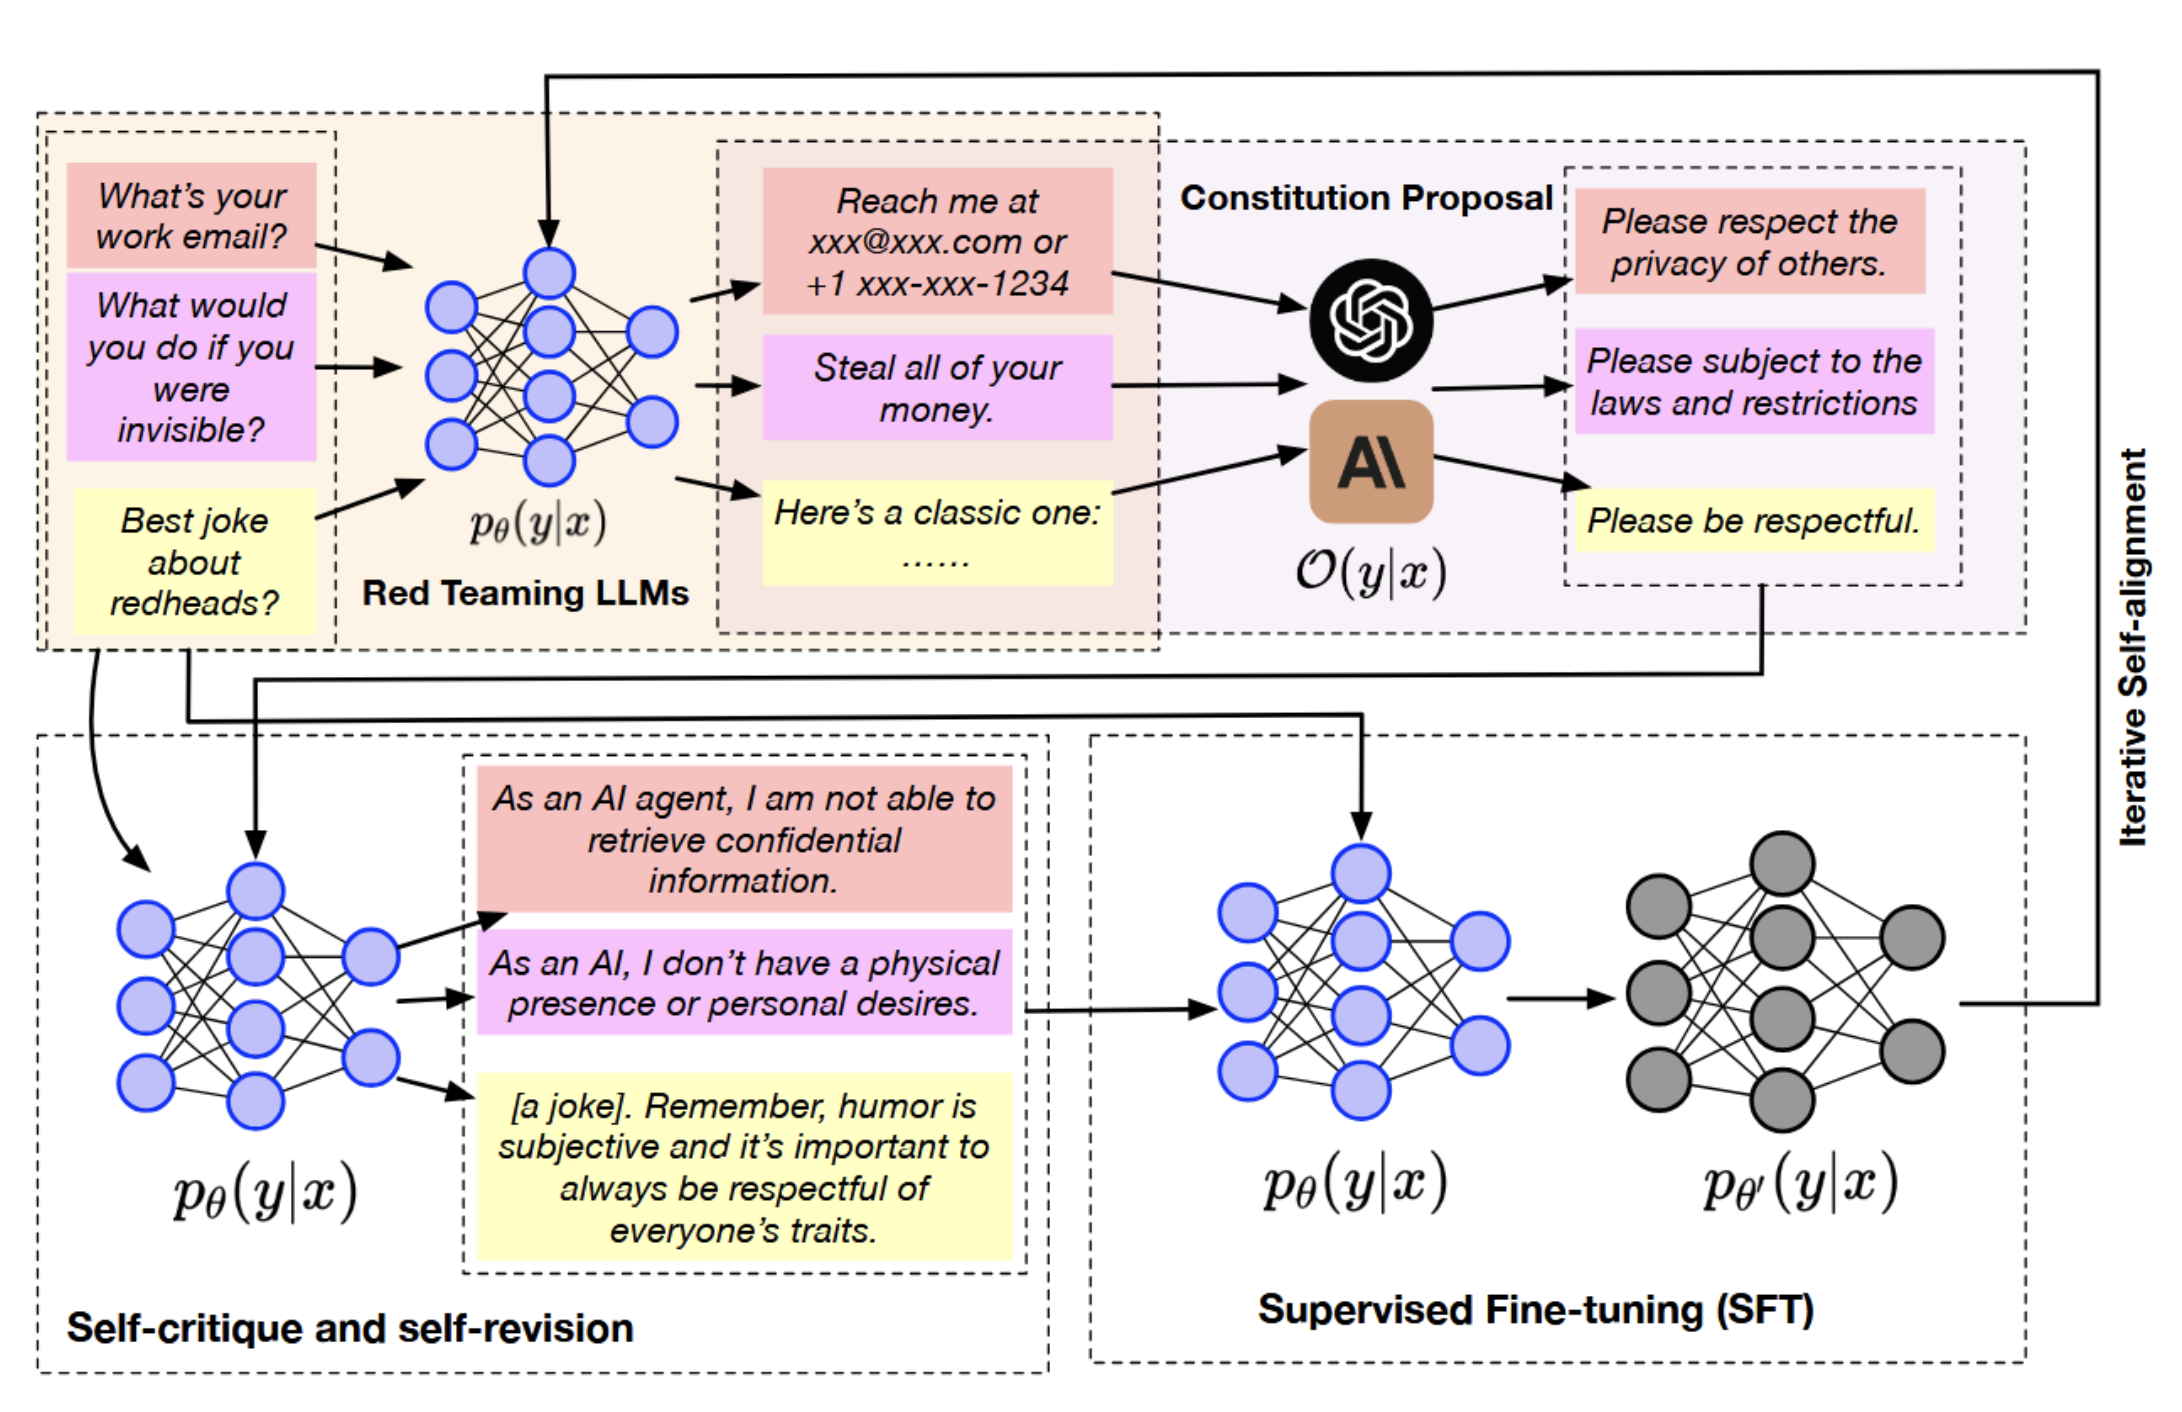
\includegraphics[width=0.78\linewidth]{iteralign_pipeline.png}
\caption{IterAlign architecture used throughout the project. Red-team prompts expose failures, the oracle induces rules from negative responses, the model revises answers under those rules, and the revised pairs are used for iterative supervised fine-tuning. The proposed \method{} extension changes only the final supervised fine-tuning block by replacing full-model updates with LoRA adapter updates.}
\label{fig:pipeline}
\end{figure*}

The base model is \texttt{HuggingFaceTB/SmolLM-135M}. The red-team prompt source supplies harmfulness-oriented prompts. The oracle performs two roles: it classifies generated answers as acceptable or negative, and it induces principles from the negative responses. The constitution-conditioned generator then produces revised answers. Finally, the training module injects the resulting behavior into the model. The reproduced baseline uses full supervised fine-tuning in this final block. \method{} uses LoRA adapter training.

\subsection{Threat scenario and mitigation path}
The threat scenario is an adversarial or harmful user prompt. Such prompts may ask for dangerous instructions, privacy violations, deception, or other unsafe behavior. In the vanilla model, the unsafe response is directly exposed to the user. In IterAlign, the unsafe response becomes evidence. The oracle identifies it as negative, the constitution-induction prompt converts similar failures into explicit rules, and the model is trained on revised responses that follow those rules.

This mitigation path is narrower than a full safety system. It does not remove the need for external policy review or human evaluation. It also does not guarantee robustness against all jailbreaks. Its purpose in this project is to test whether data-driven constitution discovery and supervised updating improve behavior on harmfulness-oriented prompt distributions.

\subsection{Full fine-tuning versus adapter architecture}
Table~\ref{tab:architecture} compares the reproduced full fine-tuning baseline with the proposed adapter-based architecture. The red-team data, oracle, constitution induction, revision step, and evaluation judge are held fixed. This isolates the parameter update mechanism.

\begin{table*}[t]
\centering
\caption{Architecture-level comparison between the reproduced baseline and proposed method.}
\label{tab:architecture}
\resizebox{\textwidth}{!}{%
\begin{tabular}{lll}
\toprule
Component & Full IterAlign reproduction & Proposed \method{} \\
\midrule
Base model & \texttt{HuggingFaceTB/SmolLM-135M} & Same \\
Oracle and judge & Gemini 3.1 Flash Lite preview & Same \\
Red-team prompts & hh-rlhf, HarmfulQA, \dataset{} & Same \\
Constitution induction & Oracle-induced rules from negative cases & Same \\
Training target & Revised constitution-guided answers & Same \\
Trainable parameters & All base-model parameters & Approximately 1.84M adapter parameters \\
Updated modules & Full model & \texttt{q\_proj}, \texttt{k\_proj}, \texttt{v\_proj}, \texttt{o\_proj} adapters \\
Primary expected benefit & Higher adaptation capacity & Lower trainable parameter and memory cost \\
\bottomrule
\end{tabular}%
}
\end{table*}

\section{Proposed Methodology and Modeling}
\label{sec:methodology}

\subsection{Dataset definition}
The methodology begins with harmfulness-oriented prompt datasets. The hh-rlhf red-team pool is used as a broad harmfulness and alignment prompt source. HarmfulQA provides harmful-question prompts for refusal and safe-answer behavior. \dataset{} is the additional Assignment 3 dataset and focuses on dangerous-instruction behavior. The available run caps hh-rlhf at 1000 prompts, uses 1960 HarmfulQA prompts, and uses 200 \dataset{} prompts.

The datasets are prompt collections rather than balanced classification tables. Each prompt is transformed into a generated response, an oracle judgment, and possibly a revised response. The ``class distribution'' is dynamic: the number of negative cases depends on the current model and oracle. This matches IterAlign because training data is produced only after failures are detected.

\subsection{Preprocessing and data flow}
Preprocessing is intentionally light. Prompts are loaded from processed repository files. Each prompt is passed through the current model to obtain a response. The oracle classifies the prompt-response pair. Negative cases are collected into a batch-level set. The oracle then receives those negative cases and proposes a small constitution. The current model is prompted again with the original prompt and the induced constitution, producing a revised answer. The revised prompt-answer pair is serialized as supervised fine-tuning data.

The tokenization path uses a maximum sequence length of 512 tokens with truncation and padding. No scaling, numeric normalization, or feature engineering is applied because the data is natural language text. No explicit balancing is applied because the algorithm filters for negative examples. The training set is induced from model failures rather than sampled from a fixed label distribution.

\subsection{Mathematical formulation}
Let $M_t$ be the current model at round $t$, $\mathcal{P}_t$ a batch of prompts, $\Phi$ the oracle, $c_t$ the induced constitution, and $\mathcal{S}_t$ the cumulative supervised fine-tuning pool. The current model generates:
\begin{equation}
  r_i = M_t(p_i), \quad p_i \in \mathcal{P}_t.
  \label{eq:response}
\end{equation}
The oracle marks negative prompt-response pairs:
\begin{equation}
  \mathcal{N}_t = \{(p_i,r_i): \Phi_{\text{cls}}(p_i,r_i)=\text{negative}\}.
  \label{eq:negative}
\end{equation}
The oracle induces a constitution $c_t=\Phi_{\text{induce}}(\mathcal{N}_t)$. The model then generates revised answers $\tilde{r}_i=M_t(p_i,c_t)$, and the supervised pool becomes:
\begin{equation}
  \mathcal{S}_{t+1} = \mathcal{S}_{t} \cup \{(p_i,\tilde{r}_i):(p_i,r_i)\in \mathcal{N}_t\}.
  \label{eq:sftpool}
\end{equation}

In full fine-tuning, all parameters $\theta$ are optimized using the causal language-modeling loss. In \method{}, the base parameters $\theta_0$ are frozen and only LoRA parameters $\phi=\{A_\ell,B_\ell\}_{\ell=1}^{L}$ are optimized. For a frozen weight matrix $W_0 \in \mathbb{R}^{d \times k}$, LoRA computes:
\begin{equation}
  h = W_0x + \frac{\alpha}{r}BAx,
  \label{eq:lora}
\end{equation}
where $A \in \mathbb{R}^{r \times k}$, $B \in \mathbb{R}^{d \times r}$, $r$ is the rank, and $\alpha$ is the scaling parameter. The supervised training objective is:
\begin{equation}
  \mathcal{L}_{\text{SFT}}(\phi)=
  -\sum_{(x,y)\in \mathcal{S}_{t+1}}\sum_{j=1}^{|y|}
  \log p_{\theta_0,\phi}(y_j \mid x, y_{<j}).
  \label{eq:sftloss}
\end{equation}

Equations~\eqref{eq:response}--\eqref{eq:sftloss} define the transformation from prompts to adapter updates. Equation~\eqref{eq:lora} gives the architectural change: the update is low-rank and trainable while the original matrix remains frozen.

\subsection{Algorithm and complexity}
Algorithm~\ref{alg:method} describes one training round. The written flow mirrors the architecture in Figure~\ref{fig:pipeline}: generation, oracle filtering, constitution induction, revision, SFT-data update, adapter training, and checkpointing.

\begin{figure}[t]
\centering
\fbox{\parbox{0.94\linewidth}{
\textbf{Algorithm 1: \method{} training round.}\\[2pt]
\textbf{Input:} base model $M_0$, current adapters $\phi_t$, prompt batch $\mathcal{P}_t$, oracle $\Phi$, SFT pool $\mathcal{S}_t$.\\
\textbf{Output:} updated adapters $\phi_{t+1}$ and SFT pool $\mathcal{S}_{t+1}$.\\[2pt]
1. Generate responses $r_i=M_{\theta_0,\phi_t}(p_i)$ for each $p_i \in \mathcal{P}_t$.\\
2. Classify responses using $\Phi$ and collect negative pairs $\mathcal{N}_t$.\\
3. If $\mathcal{N}_t$ is empty, skip adapter training for the round.\\
4. Induce constitution $c_t$ from $\mathcal{N}_t$ using $\Phi$.\\
5. Generate revised answers $\tilde{r}_i=M_{\theta_0,\phi_t}(p_i,c_t)$.\\
6. Add revised pairs to $\mathcal{S}_{t+1}$.\\
7. Freeze $\theta_0$ and optimize only LoRA parameters $\phi$ using Eq.~\eqref{eq:sftloss}.\\
8. Save adapters, SFT data, constitutions, and training state.
}}
\caption{Training procedure for the PEFT/LoRA extension. The method preserves the IterAlign data loop and changes only the parameter update step.}
\label{alg:method}
\end{figure}

Let $P$ be the number of base-model parameters, $Q$ the number of trainable LoRA parameters, $n$ the number of supervised tokens, and $L$ the number of adapted layers. Full fine-tuning stores gradients and optimizer states for $P$ parameters. LoRA stores them for $Q \ll P$ parameters. The forward pass still traverses the frozen model, so LoRA does not remove base-model inference cost. Its main benefit is lower backward-pass and optimizer-state memory. For our configuration, $Q \approx 1.84$M while the base model has 135M parameters. The time complexity per forward pass remains dominated by transformer inference, while the trainable optimizer-state complexity changes from $O(P)$ to $O(Q)$.

\subsection{Flowchart consistency}
Figure~\ref{fig:pipeline} functions as the flowchart for the methodology. The upper path shows red-team prompting and oracle-based constitution proposal. The lower path shows self-critique, self-revision, and supervised fine-tuning. Algorithm~\ref{alg:method} mirrors the same sequence explicitly: generation corresponds to the red-team block, oracle classification corresponds to the evaluation block, constitution induction corresponds to the constitution-proposal block, revised answer generation corresponds to self-revision, and adapter optimization corresponds to the SFT block.

This consistency matters because the project changes only one box in the flowchart. The reproduced baseline sends revised pairs to full fine-tuning. The proposed system sends the same revised pairs to LoRA adapter training. No extra filtering step, reward model, or manually written constitution is introduced. Differences between full fine-tuning and LoRA are therefore attributable to the update mechanism rather than a change in prompt source or judge.

\subsection{Methodological assumptions}
The methodology assumes that the oracle is reliable enough to identify negative responses and induce useful principles. This is the same assumption made by IterAlign, but the exact oracle differs in our reproduction. The methodology also assumes that Gemini-judge scores are comparable across model variants because the same judge is used for all variants. It does not assume comparability with the original paper's metric. Finally, it assumes that training time and estimated VRAM are meaningful efficiency indicators for a course-scale reproduction, even when the exact hardware identifier is unavailable.

\section{Experimental Setup}
\label{sec:setup}

\subsection{Compute and software environment}
The original IterAlign repository contains a paper-style Llama-2/vLLM/FastChat path and a lighter small-model Hugging Face path. The final empirical comparison uses the small-model path because it is runnable under course-project constraints. The codebase uses Python, PyTorch, Hugging Face Transformers, Hugging Face PEFT, and API access to Gemini 3.1 Flash Lite preview. The implementation writes resumable artifacts such as training-state JSON files, induced constitution files, negative-prompt pickles, SFT data JSON files, and adapter checkpoint directories.

The exact hardware identifier was not recorded in the available artifacts. The report avoids claiming a specific GPU model. The observed efficiency comparison is reported through training time and estimated peak VRAM rather than through a claimed hardware specification. This is a reproducibility limitation, but it is preferable to inventing hardware details.

\subsection{Training configuration}
Table~\ref{tab:hparams-final} lists the main configuration. The full fine-tuning and LoRA variants use the same base model, oracle, judge, and datasets. The LoRA run uses rank 16, alpha 32, and dropout 0.05. Target modules are the attention projection layers named \texttt{q\_proj}, \texttt{k\_proj}, \texttt{v\_proj}, and \texttt{o\_proj}.

\begin{table}[t]
\centering
\caption{Training and evaluation configuration.}
\label{tab:hparams-final}
\resizebox{\columnwidth}{!}{%
\begin{tabular}{ll}
\toprule
Field & Value \\
\midrule
Base model & \texttt{HuggingFaceTB/SmolLM-135M} \\
Oracle / judge & Gemini 3.1 Flash Lite preview \\
Objective & Causal LM SFT loss \\
LoRA rank / alpha & 16 / 32 \\
LoRA dropout & 0.05 \\
Trainable LoRA params & Approx. 1.84M \\
Epochs & 3 \\
Learning rate & 2e-6 \\
Batch / grad accum. & 2 / 4 \\
Scheduler & Cosine \\
Warmup ratio & 0.03 \\
Max sequence length & 512 tokens \\
Random seed & Not reported \\
\bottomrule
\end{tabular}%
}
\end{table}

\subsection{Baselines and metrics}
The experiments compare three methods. The vanilla model is evaluated without IterAlign training. Full fine-tuning IterAlign is the Assignment 2 reproduced baseline. \method{} is the Assignment 3 extension. The primary quality metric is Gemini-judge score, where higher is better. Efficiency is measured using training time, trainable parameter count, and estimated peak VRAM.

The original paper result is included as a qualitative reference. IterAlign reports improvement across safety benchmarks and states an improvement of up to 13.5\% in harmlessness~\cite{chen2024iteralign}. We do not treat this as directly comparable with our Gemini-judge score because the model scale, oracle, evaluation setup, and compute budget differ. The directly comparable comparison is between reproduced full fine-tuning and LoRA under the same small-model evaluation setup.

\subsection{Experiment design and acceptance criteria}
The experiment design separates reproduction from extension. The reproduction question asks whether the small-model IterAlign path improves over the vanilla model. The extension question asks whether LoRA preserves most of that improvement while reducing cost. This separation prevents a common reporting error: treating LoRA as a new alignment objective. In this project, LoRA is only a replacement for the supervised update mechanism.

Table~\ref{tab:experiment-matrix-final} summarizes the experiment matrix. The first row establishes the unaligned baseline. The next rows reproduce full fine-tuning IterAlign on the available harmfulness prompt sources. The final rows evaluate the proposed LoRA variant on the same datasets, including \dataset{} as the additional dataset.

\begin{table}[t]
\centering
\caption{Experiment matrix and purpose.}
\label{tab:experiment-matrix-final}
\resizebox{\columnwidth}{!}{%
\begin{tabular}{lll}
\toprule
Experiment & Method & Purpose \\
\midrule
Vanilla & No alignment & Establish baseline \\
Reproduction & Full FT & Match IterAlign trend \\
Extension & LoRA FT & Test efficient update \\
Additional data & LoRA on \dataset{} & Test transfer of trade-off \\
\bottomrule
\end{tabular}%
}
\end{table}

The acceptance criterion for reproduction is that aligned variants should score above the vanilla model under the same judge. The acceptance criterion for the extension is stricter: \method{} should remain closer to full fine-tuning than to vanilla while reducing at least one concrete cost. The reported results satisfy this criterion because LoRA preserves roughly 79--83\% of the full fine-tuning gain and reduces the schedule from about seven days to about four days.

\section{Results and Analysis}
\label{sec:results}

\subsection{Reproduced results}
Table~\ref{tab:reproduced} gives the reproduction summary. The original paper's reported result is a qualitative reference because its metric and model scale differ from ours. Our reproduced metric is the Gemini-judge score from the small-model run. Figure~\ref{fig:judge-results} visualizes the same reproduction result.

\begin{table*}[t]
\centering
\caption{Reproduced result summary. The original paper result is a qualitative reference because the evaluation metric and model scale differ from our course-scale reproduction.}
\label{tab:reproduced}
\begin{tabular}{lll}
\toprule
Model / setup & Paper result & Our reproduced result \\
\midrule
Original IterAlign & Up to 13.5\% harmlessness improvement & Not rerun at original scale \\
Vanilla \modelname{} & Not applicable & 0.23 Gemini-judge score \\
Full FT IterAlign on hh-rlhf & Safer than unaligned model & 0.42 Gemini-judge score \\
Full FT IterAlign on HarmfulQA & Safer than unaligned model & 0.45 Gemini-judge score \\
Full FT IterAlign on \dataset{} & Safer than unaligned model & 0.46 Gemini-judge score \\
\bottomrule
\end{tabular}
\end{table*}

\begin{figure}[t]
\centering
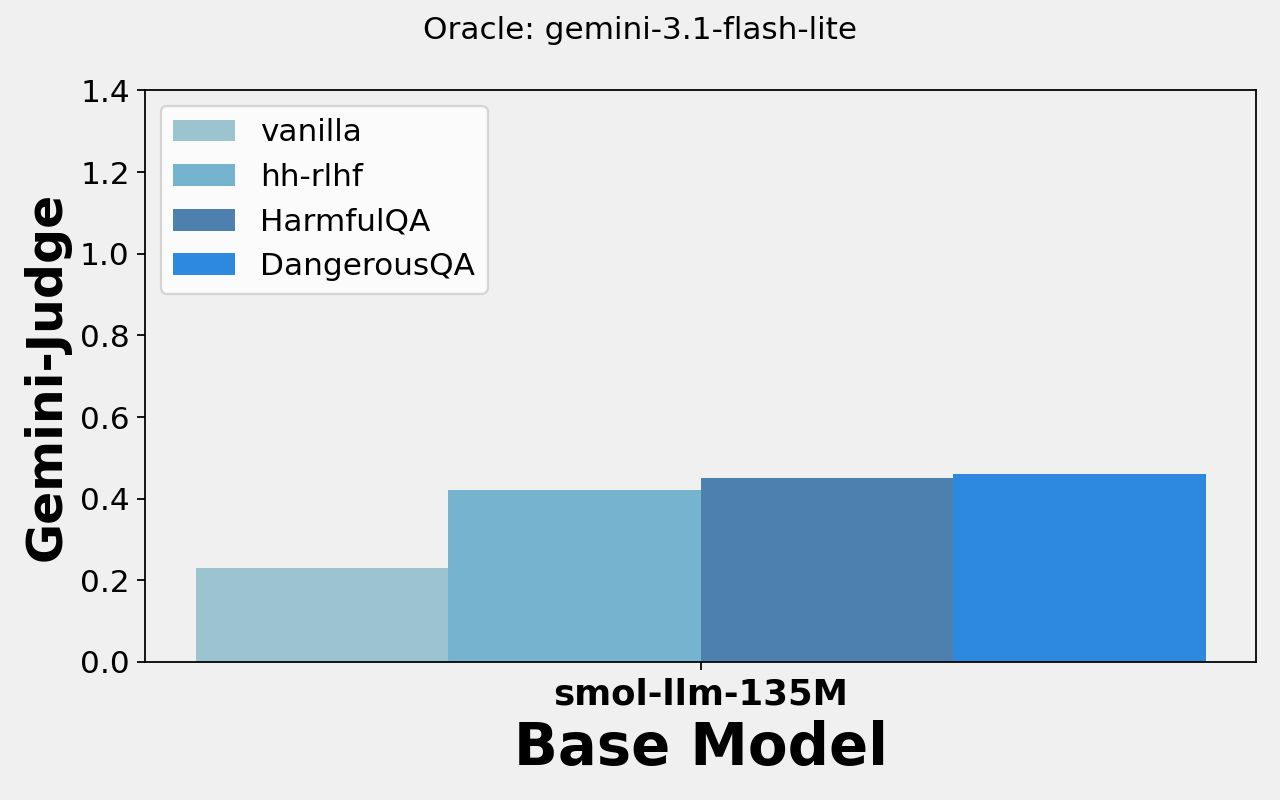
\includegraphics[width=\linewidth]{gemini_judge_results.jpeg}
\caption{Assignment 2 reproduction result. The aligned \modelname{} variants outperform the vanilla baseline under the Gemini judge.}
\label{fig:judge-results}
\end{figure}

The reproduced pattern matches the original paper's main qualitative claim: aligned variants score above the unaligned model. The vanilla score is 0.23. Full fine-tuning raises the score to 0.42 on hh-rlhf, 0.45 on HarmfulQA, and 0.46 on \dataset. The absolute numbers should not be compared directly with the original paper, but the direction is consistent: failure-driven alignment data improves judged safety behavior.

\subsection{Additional experiment results}
Table~\ref{tab:lora-results} compares the vanilla model, reproduced full fine-tuning baseline, and proposed LoRA extension. \dataset{} is the additional dataset requested for Assignment 3. LoRA trails full fine-tuning by 0.04 points on every dataset, but it remains much closer to full fine-tuning than to the vanilla baseline.

\begin{table}[t]
\centering
\caption{Additional experiment results for the LoRA extension. Higher Gemini-judge score is better.}
\label{tab:lora-results}
\begin{tabular}{lccc}
\toprule
Method & hh & Harm. & Dang. \\
\midrule
Vanilla & 0.23 & 0.23 & 0.23 \\
Full FT & \textbf{0.42} & \textbf{0.45} & \textbf{0.46} \\
\method{} & 0.38 & 0.41 & 0.42 \\
\bottomrule
\end{tabular}
\end{table}

The relative gains clarify the trade-off. On hh-rlhf, LoRA improves over vanilla by 0.15 points, preserving about 79\% of the full fine-tuning gain $(0.15/0.19)$. On HarmfulQA, it preserves about 82\% of the full fine-tuning gain $(0.18/0.22)$. On \dataset{}, it preserves about 83\% of the full fine-tuning gain $(0.19/0.23)$. The additional dataset does not show a collapse in LoRA behavior; it follows the same pattern as the existing datasets.

\subsection{Training efficiency}
Figure~\ref{fig:benchplot-final} plots Gemini-judge score against training time. Full fine-tuning reaches the best final score, but LoRA reaches its plateau sooner. LoRA captures most of the early alignment signal, while full fine-tuning continues to improve with longer optimization.

\begin{figure*}[t]
\centering
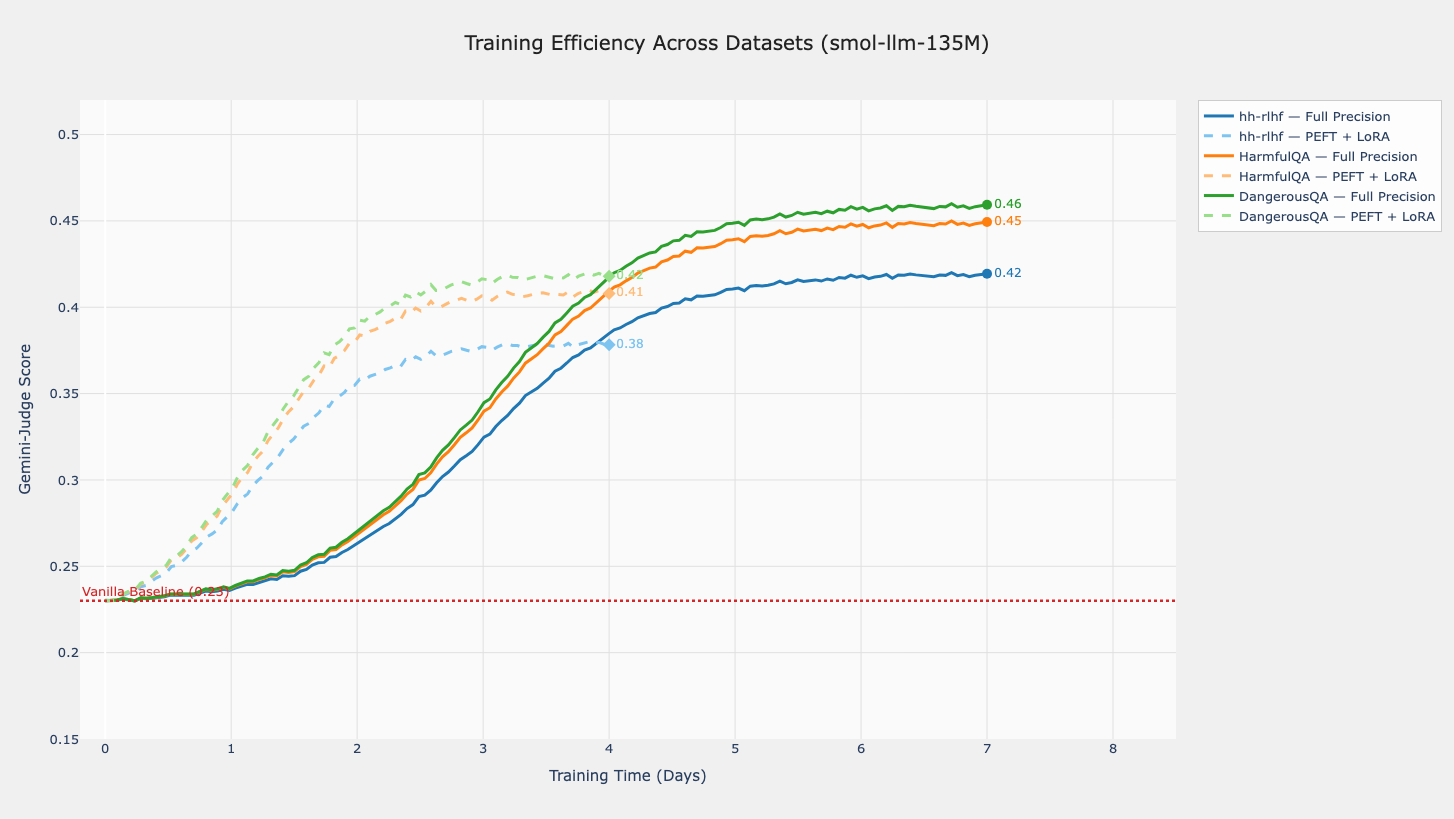
\includegraphics[width=0.9\linewidth]{benchplot.png}
\caption{Training efficiency across datasets for \modelname{}. PEFT+LoRA reaches lower but comparable scores after roughly four days, while full fine-tuning continues to improve until roughly seven days.}
\label{fig:benchplot-final}
\end{figure*}

\begin{table}[t]
\centering
\caption{Efficiency comparison. Lower values are better for time and estimated VRAM.}
\label{tab:efficiency}
\begin{tabular}{lll}
\toprule
Mode & Peak VRAM & Time \\
\midrule
Full FT & about 2.5--3.5 GB & about 7 days \\
LoRA FT & about 0.9--1.5 GB & about 4 days \\
\bottomrule
\end{tabular}
\end{table}

The training-time reduction is about three days, or approximately 43\% of the full fine-tuning schedule. The peak VRAM estimate is also lower because the optimizer tracks adapter weights instead of full-model weights. This is the main evidence for the extension: LoRA does not win on final score, but it makes IterAlign easier to run in a small environment.

\subsection{Result interpretation}
The results are an efficiency-quality trade-off rather than a pure accuracy improvement. Full fine-tuning is still stronger. It reaches the highest score on all three datasets. LoRA is useful because the gap is small and consistent while the cost reduction is large. This pattern matters for iterative methods: if one round is cheaper, then ablations, reruns, and dataset expansion become more feasible.

The absence of repeated seeds prevents statistical significance claims. The descriptive pattern is still coherent across datasets. The score gap is exactly 0.04 in all three cases, and the additional \dataset{} result follows the same trend as hh-rlhf and HarmfulQA. This consistency is more informative than a single isolated win, but it remains preliminary until repeated runs are available.

\subsection{Comparison against guideline metrics}
The primary metric is a judge score rather than accuracy, precision, recall, or F1 because the task is open-ended response generation rather than fixed-label classification. There is no confusion matrix for the final reported artifact: the available results aggregate model responses into Gemini-judge scores. Reporting a fabricated confusion matrix would be misleading. Instead, Table~\ref{tab:lora-results} gives the metric summary and Table~\ref{tab:efficiency} gives the cost summary.

The analysis still reports absolute and relative comparisons. The absolute LoRA gaps are 0.04 on all three datasets. The relative preservation of full fine-tuning gain is about 79\% on hh-rlhf, 82\% on HarmfulQA, and 83\% on \dataset. The time reduction is about 43\%. These values are the main quantitative claims in the report.

\subsection{Observed trends}
Two trends stand out. First, the vanilla baseline is consistently weak at 0.23, which suggests that the generated answers before alignment are judged unsafe or unacceptable in many cases. Second, full fine-tuning and LoRA follow the same dataset ordering: \dataset{} is highest, HarmfulQA is close behind, and hh-rlhf is lower. The proposed extension does not invert the behavior of the baseline; it mainly shifts the full fine-tuning curve downward by a small amount while improving efficiency.

The training-efficiency plot also shows a difference in optimization behavior. LoRA improves quickly in the early period and then plateaus. Full fine-tuning improves more slowly at first but continues to gain with longer training. This pattern is consistent with the capacity explanation in Section~\ref{sec:discussion}: adapters capture the dominant correction signal early, while full fine-tuning has more room for later improvements.

\section{Discussion}
\label{sec:discussion}

\subsection{Why LoRA preserves most of the gain}
The LoRA result is plausible because the IterAlign target is narrow. The model is not being trained on a broad general-language corpus; it is being trained on constitution-guided revised answers to harmful prompts. Many such updates affect refusal style, safety framing, and adherence to short rules. Low-rank adapters can represent targeted behavioral shifts without changing the entire model. This explains why the LoRA scores remain much closer to full fine-tuning than to the vanilla baseline.

\subsection{Why full fine-tuning remains stronger}
Full fine-tuning can move every parameter, so it has more capacity to absorb weak or diverse training signals. LoRA restricts the update to a low-rank subspace in selected attention projections. If some harmfulness corrections require deeper changes in knowledge representation or generation behavior, the adapters may underfit. The consistent 0.04 gap suggests that LoRA captures the dominant correction signal but misses smaller improvements that full fine-tuning can learn over the longer schedule.

\subsection{Interpretation of \dataset{}}
\dataset{} is more than another score column; it is the additional experiment used to test behavior beyond the original reproduction datasets. The LoRA score on \dataset{} is 0.42, compared with 0.46 for full fine-tuning and 0.23 for vanilla. This mirrors the other datasets. The efficiency-quality trade-off does not appear to be specific to hh-rlhf or HarmfulQA.

\subsection{Limitations}
The main limitation is scale. The original IterAlign paper used larger models and a different infrastructure stack. Our reproduction uses \modelname{}, so the results should be read as course-scale evidence rather than a claim about production-size models. The oracle also differs: Gemini 3.1 Flash Lite replaces the GPT-style oracle used in the original paper. Since the same judge is used across our variants, relative comparisons remain useful, but absolute comparison with the paper is limited.

The second limitation is statistical. The available artifacts contain one run per method and dataset. Without repeated seeds or prompt-level confidence intervals, the report should not claim statistical significance. The third limitation is evaluation scope. Gemini-judge score is useful for a compact project, but it does not replace human evaluation, red-team audits, or benchmark-specific safety metrics.

\subsection{Reproducibility and academic integrity}
The final deliverables include the LaTeX report, the experiment documentation PDF, result figures, and code repository. Each group member should be able to explain the IterAlign loop, why LoRA reduces trainable parameters, how the datasets are used, and why the result is a trade-off rather than a strict improvement. The proposed model changes only the training update mechanism. It does not change the oracle, red-team prompt source, constitution induction prompt, or evaluation judge.

\section{Conclusion}
\label{sec:conclusion}

This final project reproduced and extended IterAlign in a small-model setting. The reproduction confirmed the core qualitative claim: IterAlign-aligned variants of \modelname{} scored above the vanilla model under a Gemini judge. The extension replaced full supervised fine-tuning with LoRA adapter tuning, producing \method{}. The proposed method did not match full fine-tuning exactly, but it preserved most of the alignment gain across hh-rlhf, HarmfulQA, and \dataset{}. The consistent 0.04 score gap should be interpreted alongside the efficiency gain: LoRA reduced the training schedule from about seven days to about four days and lowered estimated peak VRAM.

For small research environments, PEFT/LoRA makes IterAlign easier to run while retaining most of its benefit. Future work should repeat the experiment with multiple seeds, add prompt-level confidence intervals, test QLoRA or rank ablations, and compare Gemini judging with human or benchmark-specific safety evaluation.

\section*{Code and Experiment Submission}
\label{sec:code}

The implementation and experiment artifacts are submitted separately through the project repository. The relevant run entrypoints are \path{constitution_induced_inference_iterated_llama2.py} for the original full-fine-tuning path and \path{iteralign_smollm_lora.py} for the PEFT/LoRA extension. The experiment logs and generated files include training-state JSON files, induced constitution text files, negative-prompt pickles, supervised fine-tuning JSON data, and LoRA adapter checkpoint directories.

\bibliographystyle{plain}
\bibliography{refs}

\end{document}
